% Use only LaTeX2e, calling the article.cls class and 12-point type.

\documentclass[12pt]{article}

% Users of the {thebibliography} environment or BibTeX should use the
% scicite.sty package, downloadable from *Science* at
% www.sciencemag.org/about/authors/prep/TeX_help/ .
% This package should properly format in-text
% reference calls and reference-list numbers.

\usepackage{scicite}

% Use times if you have the font installed; otherwise, comment out the
% following line.

\usepackage{times}

% The preamble here sets up a lot of new/revised commands and
% environments.  It's annoying, but please do *not* try to strip these
% out into a separate .sty file (which could lead to the loss of some
% information when we convert the file to other formats).  Instead, keep
% them in the preamble of your main LaTeX source file.

\usepackage{graphicx}
\usepackage{verbatim}
\usepackage{amsmath}
\usepackage{xcolor}
%\usepackage[pdfborder={0 0 0},colorlinks=false,linkbordercolor={0 0 0},urlbordercolor={0 0 0}]{hyperref}
%\usepackage[dvips, colorlinks=false, pdfborder={0 0 0}, urlcolor=blue, linkbordercolor={0 0 0},urlbordercolor={0 0 0}]{hyperref}
%\usepackage{url}
\DeclareMathOperator{\sinc}{sinc}

% The following parameters seem to provide a reasonable page setup.

\topmargin 0.0cm
\oddsidemargin 0.2cm
\textwidth 16cm 
\textheight 21cm
\footskip 1.0cm


%The next command sets up an environment for the abstract to your paper.

\newenvironment{sciabstract}{%
\begin{quote} \bf}
{\end{quote}}


% If your reference list includes text notes as well as references,
% include the following line; otherwise, comment it out.

\renewcommand\refname{References and Notes}

% The following lines set up an environment for the last note in the
% reference list, which commonly includes acknowledgments of funding,
% help, etc.  It's intended for users of BibTeX or the {thebibliography}
% environment.  Users who are hand-coding their references at the end
% using a list environment such as {enumerate} can simply add another
% item at the end, and it will be numbered automatically.

\newcounter{lastnote}
\newenvironment{scilastnote}{%
\setcounter{lastnote}{\value{enumiv}}%
\addtocounter{lastnote}{+1}%
\begin{list}%
{\arabic{lastnote}.}
{\setlength{\leftmargin}{.22in}}
{\setlength{\labelsep}{.5em}}}
{\end{list}}


% Include your paper's title here

\title{Algorithms to invert modern noble gas anomalies for the history of sea level pressure}

\author
{Geoffrey Gebbie$^{1\ast}$ \\
\\
\normalsize{$^{1}$Department of Physical Oceanography, Woods Hole Oceanographic Institution,}\\
\normalsize{360 Woods Hole Rd., Woods Hole, MA 02543, USA}\\ 
\normalsize{$^\ast$To whom correspondence should be addressed; E-mail:  ggebbie@whoi.edu.}
}

% Include the date command, but leave its argument blank.

\date{}
% start citations at the end of main body numbers. also, use original reference number from main body if a citation is duplicated (haven't figured out how to do this)
\usepackage{xpatch}
\newcounter{mybibstartvalue}
\setcounter{mybibstartvalue}{0}
%\setcounter{mybibstartvalue}{34}

\xpatchcmd{\thebibliography}{%
  \usecounter{enumiv}%
}{%
  \usecounter{enumiv}%
  \setcounter{enumiv}{\value{mybibstartvalue}}%
}{}{}

%%%%%%%%%%%%%%%%% END OF PREAMBLE %%%%%%%%%%%%%%%%


\renewcommand{\theequation}{\arabic{equation}}
\setcounter{equation}{0}

\renewcommand{\thesection}{\arabic{section}}
\setcounter{section}{0}

\begin{document} 

% Double-space the manuscript.

\baselineskip24pt

% Make the title.

\maketitle 

% Place your abstract within the special {sciabstract} environment.

\begin{sciabstract}
\end{sciabstract}

% In setting up this template for *Science* papers, we've used both
% the \section* command and the \paragraph* command for topical
% divisions.  Which you use will of course depend on the type of paper
% you're writing.  Review Articles tend to have displayed headings, for
% which \section* is more appropriate; Research Articles, when they have
% formal topical divisions at all, tend to signal them with bold text
% that runs into the paragraph, for which \paragraph* is the right
% choice.  Either way, use the asterisk (*) modifier, as shown, to
% suppress numbering.

\section{Overview} 

% In this section, we present an overview of the methods.
This text provides supporting information regarding numerical methods
to invert modern oceanic noble gas anomalies for a timeseries of sea level pressure.

\subsection{Ocean circulation links between temporal and spatial variability}
\label{sec:hist-surf-vari}

Ocean tracers, including noble gas concentrations, carry the imprint
of surface conditions into the subsurface ocean, making a record of
past surface conditions in today's ocean. Surface conditions are
transported to some parts of the subsurface ocean faster than others,
and therefore past temporal variability leads to spatial variability
in any snapshot of the ocean. Even globally-uniform changes at the
surface will lead to subsurface gradients through this mechanism
\cite{Scheen-Stocker-2020:Effect,Gebbie-Huybers-2019:Little}.

We observe a noble gas difference between $35^{\circ}$N and
$10^{\circ}$S along the meridional section at $150^{\circ}$W and 3.5
km depth. This difference is isolated to a $p_{\star}=2.8 \pm 0.4$
mbar sea level pressure difference during the formation of the waters,
where $p_{\star}$ is the influence of pressure at the time that water
leaves the surface mixed layer which is conservative in the
subsurface. We suggest the notation $p_{\star}$ or ``preformed
pressure'' in analogy with $\mathrm{P}_{\star}$, the preformed phosphate
\cite{IOC-2010:TEOS}. If these two locations have waters with
sufficiently different ages, or elapsed time since water was last at
the surface, the difference could be explained by the timing of past
surface changes.

Here we calculate the age distributions for representative abyssal
North and South Pacific sites from an empirically-derived steady-state
ocean circulation model that fits modern-day climatological
distributions of temperature, salinity, phosphate, nitrate, oxygen,
oxygen-isotope ratio, and radiocarbon
\cite{Gebbie-Huybers-2012:mean}. Both sites have waters with a wide
range of ages from a few hundred to a few thousand years (Figure 1)
because of the many routes from abyssal water formation sites and the
significant time for mixing to occur
\cite{Khatiwala-Visbeck-2001:Age}. The age distributions are peaked at
about 800 and 1000 years for the South and North Pacific sites,
respectively, indicating that the South Pacific has waters of a
younger age due to being closer to Antarctic sites of abyssal water
formation. Although abyssal Pacific waters move slowly and remain in
the basin for a long time, there are clear meridional differences in
the ages of seawater.
 
\begin{figure}[htbp]
 \begin{center}
 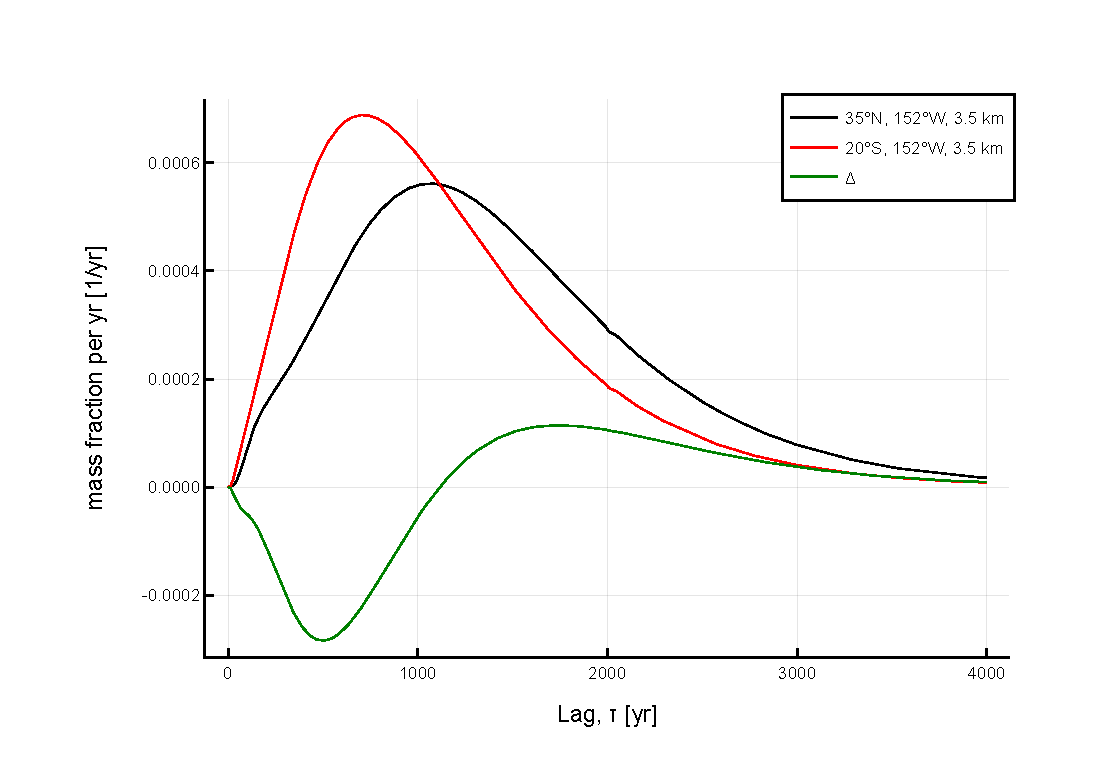
\includegraphics[scale=0.9]{../plots/deltaresponse_NPACvSPAC.pdf} \\
 \noindent{{\bf Figure 1. Age distributions from the North
     (\textit{black}) and South (\textit{red}) Pacific along
     $152^{\circ}W$ and 3.5 km depth, as well as the north minus south
     difference (\textit{green}), as calculated from an
     empirically-derived ocean circulation model.} The integral under
   the black and red curves is such that the total mass fraction is
   unity. Lags on the x-axis refer to the time lag of subsurface
   signals relative to the surface.}
 \end{center} 
\end{figure}

The preformed pressure value today (i.e., 2023 CE) at the North
Pacific sample location $r_{np}$ is related to the past via a
convolution equation,
\begin{equation}
\label{eq:2}
p_{\star}(2023~ \mathrm{CE}, r_{np}) = \sum_{i=1}^{3000} g_i(r_{np})~  p_{\star}(2023~ \mathrm{CE} - i~\mathrm{yr}, r_{b}),
\end{equation}
which is a sum of contributions from $g_i$, the annually-resolved age
distribution, operating on the past surface boundary conditions at
$r_b$ \cite{Hall-Haine-2002:ocean}.  The distribution is denoted $g_i$
to recall the discrete-time Green's function, and is available from
the steady-state circulation for the past 4,000 years. The sum of
$g_i$ values is greater than 0.99 indicating that 4,000 years is
sufficient to capture over 99\% of the age distribution. Note that
$g_{i}$ is dimensionless and has been translated into a mass fraction
per year to be displayed in continuous, rather than discrete, form in
Figure 1. A similar equation is available for the South Pacific
location.

The difference between the North and South Pacific age distributions
is key for mapping time variability into space. The difference between
equation~(\ref{eq:2}) and an equivalent South Pacific equation yields
a constraint on the preformed pressure difference:
\begin{equation}
\label{eq:3}
{\Delta}p_{\star}(2023~ \mathrm{CE}, r_{np}, r_{sp}) = \sum_{i=1}^{4000} {\Delta}g_i~  p_{\star}(2023~ \mathrm{CE} - i~\mathrm{yr}, r_{b}),
\end{equation}
where ${\Delta}p_{\star}$ is the north minus south preformed pressure
difference and the new Green's function is a difference (i.e.,
${\Delta}g_i = g_{i}(r_{np}) - g_{i}(r_{sp})$ where $r_{sp}$ refers to
the South Pacific location. This equation is simplified under the
assumption that the Green's functions are unchanging in time, an
assumption that appears to be true to first order given the slight
modifications to ocean hydrographic structure over the past 150 years
\cite{Gebbie-Huybers-2019:Little}. It is also assumed that past
changes in preformed phosphate are globally-uniform, which is clearly
untrue and will be interpreted later in this document. In concept,
equation~(\ref{eq:3}) relates a spatial gradient on the left hand side
to a surface timeseries on the right hand side.

The north-south difference in age distributions shows negative values
around 500 years and positive values around 1,500 years (green, Figure
1), as is possible because differences of distributions are no longer
required to be non-negative. If surface conditions imprinted the
signal of higher pressure 500 years ago, it would be reflected with
South Pacific preformed pressure being higher than the North
Pacific. What is actually observed is the North Pacific being higher
than the South, suggesting that surface conditions had lower pressure
500 years ago. Any timeseries of surface changes that projects on
${\Delta}g_i$, however, also affect today's meridional gradient in
$p_{\star}$, and a quantitative method is required to sort through the
range of plausible solutions.

Another concern is whether ocean mixing would erase the signal of past
surface conditions before they could be recorded today. The magnitude
and shape of the curve that represents ${\Delta}g_i$ in Figure 1
contains information about this mixing and damping of surface signals
through time. In some sense, ${\Delta}g_i$ is analogous to an ocean
circulation filter which acts to transform the surface
timeseries. Thus, any quantitative method must be able to perform a
de-convolution to determine whether north-south age differences are
large enough to explain the observed preformed-pressure spatial
gradient.

\subsection{Seawater vintages}

It is highly unlikely that noble gases contain information about
year-to-year to even decade-to-decade changes. Therefore, we simplify
the analysis by defining vintages of seawater that describe the epoch
during which water was last at the surface. Vintages have previously
been used to describe the year that waters left the surface
\cite{Pickart2002}, like a vintner describes a batch of wine, and here
we use the term for a much wider range of years. Here we define the
following vintages: modern (MOD, 1800 - 2022 CE), Little Ice Age (LIA,
1300- 1800 CE), Medieval Climate Anomaly (MCA, 800 - 1300), Dark Ages
Cold Period (DACP, 300 -800 CE), Roman Warm Period (RWP, 200 BCE - 300
CE), and the pre-Roman Warm Period (preRWP, before 200 BCE). Note that
these time intervals do not strictly match definitions in the
literature \cite{Paasche-Bakke-2010:Defining}, but instead are chosen
to prioritize 500-year intervals for ease of later interpretation.

The description of the waters that bathe the North and South Pacific
sites can now be simplified to the combination of these six vintages. The mass fraction of each vintage is calculated by integrating the age distribution over the appropriate time interval, for example for the Little Ice Age (LIA),
\begin{equation}
\label{eq:3}
m_{LIA}(r_{np}) = \sum_{i=2023-1800}^{2023-1300} g_i(r_{np}),
\end{equation}
where $m_{LIA}$ is the mass fraction of LIA water and the time indices
account for the time elapsed between the LIA and today.  Following the
development above, the key relationship between temporal and spatial
gradients is simplied,
\begin{equation}
\label{eq:3}
{\Delta}p_{\star}(2023~ \mathrm{CE}, r_{np}, r_{sp}) = \sum_{j=1}^{6} {\Delta}m_j~  p_{\star}(j, r_{b}),
\end{equation}
where the summation include six vintages, the mass-fraction difference
is ${\Delta}m_j = m_{j}(r_{np}) - m_{j}(r_{sp})$, and the history of
surface boundary conditions is identified with a particular climate
epoch. This simplification makes a tradeoff; it will be more difficult
to explain the observations but all solutions will represent a
realistic system with centennial-scale changes in climate.


\subsection{Inverse problem}

Equation~(\ref{eq:3}) represents an underdetermined problem with one
constraint, six unknowns, and infintely-many solutions. Here we
provide information regarding the expected covariance of the solution
to construct a statistical solution with its uncertainty. The solution
method, detailed next, is based on the Gauss-Markov Theorem
\cite{Wunsch-2006:Discrete}.

For ease of notation we collate the unknown parameters and the vintage mass fractions into vectors:
\begin{equation}
  \mathbf{x} = \left(\begin{array}{c}  p_{\star}(\mathrm{MOD}, r_{b}) \\
                          p_{\star}(\mathrm{LIA}, r_{b}) \\
                          p_{\star}(\mathrm{MCA}, r_{b}) \\
                          p_{\star}(\mathrm{DACP}, r_{b}) \\
                          p_{\star}(\mathrm{RWP}, r_{b}) \\
                          p_{\star}(\mathrm{preRWP}, r_{b}) 
                        \end{array} \right),
                      \end{equation}
                      and
                      \begin{equation}
                        \mathbf{m} = \left(\begin{array}{c}  {\Delta}m_{MOD} \\
{\Delta}m_{LIA} \\
{\Delta}m_{MCA} \\
{\Delta}m_{DACP} \\
{\Delta}m_{RWP} \\
{\Delta}m_{preRWP} 
 \end{array} \right) .
\end{equation}
Now the constraint is symbolically described as,
\begin{equation}
\label{eq:4}
y = \mathbf{m}^{T}\mathbf{x} + \mathbf{n},
\end{equation}
where the observation is $y={\Delta}p_{\star}(2023~ \mathrm{CE}, r_{np}, r_{sp})$, \textit{T} is the vector transpose, and $\mathbf{n}$ is a reminder that the observational fit is not expected to be perfect.

The Gauss-Markov Theorem provides a means to solve an underdetermined problem via the solution formula, 
\begin{equation}
\label{eq:5}
{\tilde {\bf x}} = {\bf C}_{xx} {\bf m} (\mathbf{m}^{T}{\bf C}_{xx} {\bf m} + {\bf C}_{nn})^{-1} y
\end{equation}
which is valid so long as the quantity in parentheses is invertible. We denote $\mathbf{\tilde{x}}$ with a tilde to mark that it is a solution. The observation $y$
is not bold because it is a scalar, not a vector. This solution satisfies a number of advantageous statistical properties, such as being unbiased and minimizing the uncertainty of each solution element. Such properties only hold in the case that the input statistical information, the solution and observation covariance matrices $\mathbf{C}_{xx}$ and $C_{nn}$ are valid. 

The observational covariance is easily set as it is the observational
variance: $C_{nn} = (0.4 \mathrm{mbar})^{2}$. The solution covariance has two components: 1) setting the baseline or reference for the preformed pressure anomalies, and 2)
a description of the expected climate variability.
Here we define the reference for the anomalies to be the pre-industrial (all vintages but MOD) $p_{\star}$ average. Such a constraint could be added to the system as a second observational equation of the form:
\begin{equation}
\label{eq:7}
\bar{p_{\star}} = \sum_{j=2}^{6} ~\frac{1}{5}  p_{\star}(j, r_{b}) = \mathbf{\overline{m}}^{T} \mathbf{x} = 0,
\end{equation}
where $(1 /5)$ arises from the average over five vintages. Instead we recognize that this constraint imposes a covariance of the form, $\mathbf{C}_{xx} = \sigma^{2 }\mathbf{\overline{m}}^{T} \mathbf{\overline{m}}$, where $\sigma$ is the expected deviation from a perfect zero reference level. Here we choose the small but non-zero value of $\sigma=10^{-4}$ mbar.

For part (2) of the solution covariance, we experiment with three cases with increasing complexity.
\begin{itemize}
\item Minimum variance of solution

  We define the solution covariance to conservatively assume that $p_{\star}$ has a standard deviation of 10 mbar based upon existing sea level pressure gradients and
  historical model simulations \cite{Hakim-Emile-Geay-2016:last}. All epochs are assumed to vary independently. The solution covariance is
  
\begin{equation}
\label{eq:6}
\mathbf{C}_{xx} = \left(
\begin{array}{cccccc}
100.0 & 0.0 & 0.0 & 0.0 & 0.0 & 0.0 \\
0.0 & 100.0 & 0.0 & 0.0 & 0.0 & 0.0 \\
0.0 & 0.0 & 100.0 & 0.0 & 0.0 & 0.0 \\
0.0 & 0.0 & 0.0 & 100.0 & 0.0 & 0.0 \\
0.0 & 0.0 & 0.0 & 0.0 & 100.0 & 0.0 \\
0.0 & 0.0 & 0.0 & 0.0 & 0.0 & 100.0 \\
\end{array}
\right) \mathrm{mbar}^{2}
\end{equation}
The solution covariance from (1) that defines the anomaly reference level is added to this matrix, as is done in all cases to follow.

\item Minimum trend

  The climate epochs are several hundred years long but the climate is
  known to have variability at these scales and longer. In this second
  case, we define the solution covariance such that trends have an
  expected magnitude no larger than $p\prime = 4$ mbar/century based
  upon the few long timescale climate frequency spectra that are
  available \cite{Huybers-Curry-2006:Links}. We define a matrix $\mathbf{D}$ that calculates differences between all combinations of vintages, and where the expected output for vintages $i$ and $j$ is:
  \begin{equation}
\label{eq:8}
{\Delta}p_{\star}(i,j) = p\prime {\Delta}t(i,j)
\end{equation}
where ${\Delta}t(i,j)$ is the time difference between the midpoints of vintages $i$ and $j$. 
The resulting covariance matrix is $\mathbf{D}\mathbf{D}^{T}$ where each element is scaled by $(1 / {\Delta}p_{\star}(i,j))^{2}$.

\item Combined covariance matrix

  The combined covariance matrix (labeled ``min-trend-variance'') is a
  sum of the covariance from (1) the definition of the reference level
  for preformed pressure anomalies, 2) the expected variance of
  preformed pressure about this reference level (``min-variance''),
  and 3) expectation of correlation between vintages that are adjacent
  in time (``min-trend'').
  
\end{itemize}

\subsection{Inverse solutions}

The three inverse solutions use a variety of statistical input from
different information sources but converge to a common solution
between the Little Ice Age and Roman Warm Period (2,000 and 500 years
ago (Figure 2). This time period is marked by a
statistically-significant ($p=0.05$) inferred decrease of sea level
pressure by $17 \pm 8$ mbar. The solutions also have common elements
prior to 1,500 years ago.  The greatest differences come in relation
to LIA to modern changes. Because seawater in the abyssal North
Pacific has very little modern vintage water, we are unable to
conclusively place modern sea level pressure in context of previous
changes. It is possible that modern sea level pressure is about the
same as the LIA, or it could be as much as 15 mbar higher.

\begin{figure}[htbp]
 \begin{center}
 \includegraphics[scale=0.9]{../plots/SLP_CommonEra_combined.pdf} \\
 \noindent{{\bf Figure 2. Inferred historical sea level pressure
     variations.} All results use the identical noble gas
   observational information, but differ in the assumed solution
   covariance matrix (blue: min-trend, red: min-variance, green:
   min-trend-variance). Error ribbons represent the $1\sigma$ uncertainty
   level. Results from each vintage are plotted as a single value at
   the midpoint of the interval.} \end{center}
\end{figure}

The problem formulation has proceeded by assuming that sea level
pressure changes are globally-uniform, but such large changes in sea
level pressure would indicate a change in the mass of the
atmosphere. The low solubility of nitrogen and oxygen in seawater make
such large mass changes unlikely. Instead, the results of the inverse
solution should be interpreted in a more nuanced way. Signals in
abyssal waters primarily reflect surface signals at the sites of
formation in polar oceans, and we lack direct information about the
tropics and subtropics here. Thus, inferred changes in the LIA and
earlier should be interpreted as changes in polar oceans, and
constraints on the global mass of the atmosphere can be balanced by
opposing changes in the tropics.

It is still debated whether the LIA is a North Atlantic-centric or
global phenomenon. Our inferences of sea level pressure change are
best interpreted as changes in polar regions and cannot directly be
pinpointed as northern or southern hemisphere variability. Due to the
water-mass composition of the abyssal Pacific being dominated by
southern source waters, however, we suggest that the noble gas signal
is more easily explained by changes in and around Antarctica. North
Atlantic waters occupy less than half the mass of Antarctic waters in
the abyssal North Pacific \cite{Johnson--2008:Quantifying}, and would
require an sea level pressure signal that is more than twice as large
(30+ mbar) if the Antarctic region did not participate in the LIA.

\subsection{Sea-level pressure differences between climate eras}
\label{sec:slp-differences}

 \begin{table}
\label{tab:slp-differences}
   \caption{Sea-level pressure differences in millibars between
     climate eras, as defined by the difference of the value during
     one vintage (\textit{rows}) and another vintage
     (\textit{columns}) calculated in the min-trend-variance
     case. Some differences are significant at the 67\%
     (\textbf{bold}) and 95\% (\textcolor{red}{\textbf{{bold, red}}}) confidence
     levels. The vintages are: modern (MOD, 1800 - 2022 CE), Little
     Ice Age (LIA, 1300- 1800 CE), Medieval Climate Anomaly (MCA, 800
     - 1300), Dark Ages Cold Period (DACP, 300 -800 CE), Roman Warm
     Period (RWP, 200 BCE - 300 CE), and the pre-Roman Warm Period
     (preRWP, before 200 BCE). }
   \centering {\small
\begin{tabular}{l|cccccc}
\hline
Vintage  & MOD & LIA & MCA & DACP & RWP & pre-RWP  \\
\hline
%\left[
%\begin{array}{cccccc}
MOD & 0.0 ± 0.0  & 5.1 ± 7.2  & -0.78 ± 8.9  & -8.3 ± 8.6  & \bf{-10.9 ± 8.3}  & \bf{-13.5 ± 8.2}  \\
LIA & -5.1 ± 7.2  & 0.0 ± 0.0  & -5.8 ± 7.9  & \textcolor{red}{\bf{-13.4 ± 6.7}}  & \textcolor{red}{\bf{-16.0 ± 6.1}}  & \textcolor{red}{\bf{-18.5 ± 5.6}}  \\
MCA & 0.8 ± 8.9  & 5.8 ± 7.9  & 0.0 ± 0.0  & -7.5 ± 7.8  & \bf{-10.2 ± 8.1}  & \bf{-12.7 ± 8.3}  \\
DACP & 8.3 ± 8.6  & \textcolor{red}{\bf{13.4 ± 6.7}}  & 7.5 ± 7.8  & 0.0 ± 0.0  & -2.6 ± 8.5  & -5.1 ± 9.5  \\
RWP & \bf{10.9 ± 8.3}  & \textcolor{red}{\bf{16.0 ± 6.1}}  & \bf{10.2 ± 8.1}  & 2.6 ± 8.5  & 0.0 ± 0.0  & -2.5 ± 9.0  \\
pre-RWP & \bf{13.5 ± 8.2}  & \textcolor{red}{\bf{18.5 ± 5.6}}  & \bf{12.7 ± 8.3}  & 5.1 ± 9.5  & 2.5 ± 9.0  & 0.0 ± 0.0  \\ 
%\end{array}
  % $l1$  & 260   \\
  % $l2$  & 300   \\
  % $l3$  & 340   \\
  % $h1$  & 270   \\
  % $h2$  & 250   \\
  % $h3$  & 380   \\
  % $r1$  & 370   \\
  % $r2$  & 390   \\
\hline
%\multicolumn{2}{l}{$^{a}$Footnote text here.}
\end{tabular}}
\end{table}

% A table for min-trend-variance case.
% \begin{equation}
% \left[
% \begin{array}{cccccc}
% 0.0 ± 0.0 mbar & 5.1 ± 7.2 mbar & -0.78 ± 8.9 mbar & -8.3 ± 8.6 mbar & -10.9 ± 8.3 mbar & -13.5 ± 8.2 mbar \\
% -5.1 ± 7.2 mbar & 0.0 ± 0.0 mbar & -5.8 ± 7.9 mbar & -13.4 ± 6.7 mbar & -16.0 ± 6.1 mbar & -18.5 ± 5.6 mbar \\
% 0.78 ± 8.9 mbar & 5.8 ± 7.9 mbar & 0.0 ± 0.0 mbar & -7.5 ± 7.8 mbar & -10.2 ± 8.1 mbar & -12.7 ± 8.3 mbar \\
% 8.3 ± 8.6 mbar & 13.4 ± 6.7 mbar & 7.5 ± 7.8 mbar & 0.0 ± 0.0 mbar & -2.6 ± 8.5 mbar & -5.1 ± 9.5 mbar \\
% 10.9 ± 8.3 mbar & 16.0 ± 6.1 mbar & 10.2 ± 8.1 mbar & 2.6 ± 8.5 mbar & 0.0 ± 0.0 mbar & -2.5 ± 9.0 mbar \\
% 13.5 ± 8.2 mbar & 18.5 ± 5.6 mbar & 12.7 ± 8.3 mbar & 5.1 ± 9.5 mbar & 2.5 ± 9.0 mbar & 0.0 ± 0.0 mbar \\
% \end{array}
% \right]
% \end{equation}


% Unfortunately, the table is missing labels. This is for the ``min$_{trend}$'' experiment.n


% \begin{equation}
% \left[
% \begin{array}{cccccc}
% 0.0 ± 0.0 mbar & 1.6 ± 9.2 mbar & -3.9 ± 12.0 mbar & -11.0 ± 12.0 mbar & -15.0 ± 11.0 mbar & -18.0 ± 11.0 mbar \\
% -1.6 ± 9.2 mbar & 0.0 ± 0.0 mbar & -5.5 ± 10.0 mbar & -12.6 ± 8.9 mbar & -16.7 ± 7.5 mbar & -20.1 ± 7.1 mbar \\
% 3.9 ± 12.0 mbar & 5.5 ± 10.0 mbar & 0.0 ± 0.0 mbar & -7.1 ± 9.6 mbar & -11.0 ± 10.0 mbar & -15.0 ± 11.0 mbar \\
% 11.0 ± 12.0 mbar & 12.6 ± 8.9 mbar & 7.1 ± 9.6 mbar & 0.0 ± 0.0 mbar & -4.1 ± 11.0 mbar & -7.5 ± 13.0 mbar \\
% 15.0 ± 11.0 mbar & 16.7 ± 7.5 mbar & 11.0 ± 10.0 mbar & 4.1 ± 11.0 mbar & 0.0 ± 0.0 mbar & -3.4 ± 12.0 mbar \\
% 18.0 ± 11.0 mbar & 20.1 ± 7.1 mbar & 15.0 ± 11.0 mbar & 7.5 ± 13.0 mbar & 3.4 ± 12.0 mbar & 0.0 ± 0.0 mbar \\
% \end{array}
% \right]
% \end{equation}

The scenario with the highest degree of sophistication is labeled ``min-trend-variance.''
The long-term trend between the Little Ice Age and the earliest climate eras (Dark Ages Cold Period, Roman Warm Period, and pre-Roman Warm Period) is significant at the 95\% confidence level (Table~\ref{tab:slp-differences}). In particular, we estimate that the pre-RWP to LIA decrease 
of $19 \pm 11$ mbar ($2\sigma$ error bars) is well constrained by the data.
Differences over shorter time periods are generally not significant. It is also difficult to find a significant relation to modern sea level pressures.

% Our goal is to extract the decadal signal of water-mass change from
% the historical temperature observations.  The historical-to-WOA
% temperature difference is computed by interpolating the World Ocean
% Atlas values onto the historical data locations. The historical-to-WOA
% temperature difference profile is computed by a least-squares method
% that accounts for contamination by measurement error and signals that
% are not representative of the decadal-mean, basinwide-average
% temperature. The contamination is assumed to have three parts: (1)
% transient effects such as isopycnal heave due to internal waves or
% mesoscale eddies, (2) irregular spatial sampling of each basin, and
% (3) measurement or calibration error of the thermometer.  The expected
% size of (1) is taken from the WGHC error estimates and depends upon
% location.  Following \cite{Huang--2015:Heaving}, the variance due to
% (2) is assumed to be $20\%$ that of (1), and the standard error due to
% (3) is assumed equal to $0.14^{\circ}$C
% \cite{Roemmich-Gould-2012:135}.


% \subsection{Vertical profile of temperature difference}

% The temperature difference between the historical observations and the
% corresponding World Ocean Atlas (WOA) value is,
% \begin{equation}
% \Delta T(r_i) = T(r_i,t_w) - T(r_i,t_h),
% \end{equation}
% where $T(r_i,t_h)$ is the $i$th {\it historical} temperature
% observation at location, $r_i$, and time, $t_h$, and $T(r_i,t_w)$ is
% the WOA temperature at the same location. The observations are
% combined into a vector,
% \begin{equation}
% {\boldsymbol \Delta}{\bf T} = \left(\begin{array}{c} \Delta T(r_1) \\
%                                       \Delta T(r_2) \\ \vdots \\
%                                       \Delta T(r_M) 
%  \end{array} \right) .
% \end{equation}
% Temperature changes at a given pressure are assumed equivalent to potential temperature changes.

% \subsection{Basinwide-average temperature profiles}

% Our goal is to extract the decadal signal of water-mass change from
% the historical temperature observations 
% \begin{equation}
% \overline{{\boldsymbol \Delta}{\bf T}} = \left(\begin{array}{c} \overline{\Delta \theta(z_1)}
%                   \\\overline{\Delta \theta(z_2)} \\ \vdots \\ \overline{\Delta \theta(z)_K} 
%  \end{array} \right),
% \end{equation}
% where we have defined a grid of $K$ depths.  Given knowledge of the
% basinwide averages, one can make a prediction for each WOA$-$historical temperature difference,
% \begin{equation}
% {\boldsymbol \Delta}{\bf T} = {\bf V}\overline{{\boldsymbol \Delta}{\bf T}} + {\bf q},
% \end{equation}
% where ${\bf V}$ maps the basinwide mean onto the observational point
% by noting the basin of the observations and vertical linear
% interpolation, ${\bf q}$ is contamination by measurement error and
% signals that are not representative of the decadal-mean,
% basinwide-average temperature. The contamination is decomposed into
% three parts,
% \begin{equation}
% {\bf q} = {\bf n}_T + {\bf n}_S + {\bf n}_M,
% \end{equation}
% where ${\bf n}_T$ is contamination by transient effects such as
% isopycnal heave due to internal waves or mesoscale eddies, ${\bf n}_S$
% is due to the irregular spatial sampling of each basin, and
% ${\bf n}_M$ is measurement or calibration error of the
% thermometer. Note that no depth correction is made here, and
% temperature differences may be biased toward warming.

% The expected size of ${\bf n}_T$ is related to the energy in the
% interannual and higher-frequency bands. We use estimates from the WOCE
% Global Hydrographic Climatology \cite{Gouretski-Koltermann-2004:WOCE}
% to quantify this error and its spatial pattern.  Errors that primarily
% reflect an uncertainty due to a representativity error were previously
% estimated in this climatology, where the magnitude of interannual
% temperature variability is $1.6^{\circ}$C at the surface, decreasing
% to $0.8^{\circ}$C below the mixed layer, and $0.02^{\circ}$C at 3000
% meters depth. Inherent in their mapping is a horizontal lengthscale of
% $L_{xy}^{T}=450$ km. This corresponds to a vertical lengthscale of
% $L_z^{T}=450$ meters when applying an aspect ratio based upon mean
% depth and lateral extent of the ocean. Their mapping is the degree of
% error necessary to place the non-synoptic cruises of a 10-year time
% interval into a coherent picture. Estimated errors are similar to
% those of \cite{Wortham-Wunsch-2014:multidimensional}, who also note
% that the spatial scales increase as the temporal scales
% increase. Above 1300 meters depth, the aliased variability is
% typically larger than the measurement error described below.

% Next we describe the second moment matrix of temporal contamination,
% ${\bf R}_{TT} =<{\bf n}_T ({\bf n}_T)^T>$. Note that ${\bf n}_T$
% depends on the difference of contamination during the two time
% periods, $n_T(r_i) = \eta_T(r_i,t_w) - \eta_T(r_i,t_h)$, where
% $\eta_T(r,t)$ is the difference between temperature at a given time
% and the decadal average. The WGHC statistics give the error covariance
% for $\eta_T(r,t_w)$ not $n_T(r)$. This covariance matrix is
% reconstructed by first creating a correlation matrix,
% \begin{equation}
%   {\bf R}_{\rho} = \left(\begin{array}{ccccc}
% \rho(0) & \rho(\delta) & \rho(2\delta) & \hdots & \\
% \rho(\delta) & \rho(0) & \rho(\delta) & \hdots &  \\    
% \rho(2\delta) & \rho(\delta) & \rho(0) & \hdots &  \\    
% \vdots &   \vdots           &  \vdots       &    \ddots & \\
% &              &         &     & \rho(0) \end{array} \right),
% \end{equation}
% where the autocorrelation function, $\rho(\delta)$, is given by a
% Gaussian with a horizontal lengthscale of 450 km and a vertical
% lengthscale of 450 meters. We derive the covariance matrix by
% weighting the correlation matrix,
% ${\bf R}_{\eta\eta} = {\boldsymbol \sigma}_\eta {\boldsymbol
%   \sigma}_\eta^T \circ {\bf R}_{\rho} $, where
% ${\boldsymbol \sigma}_\eta$ is the vector of the standard deviation of
% the WGHC interannual variability and $\circ$ is the Hadamard
% product. Here the time interval of the historical cruises is about 20
% years, or twice as long as the WOCE era. Due to the red spectrum of
% ocean varabilility, the potential for aliased variability over this
% longer time interval is increased. To get a better constraint on
% $T_{ratio}$, we have to assume a frequency spectrum. If we assume the
% power density spectrum is red with a power law of $f^{-2}$, then we
% can integrate to determine the variance at frequencies greater than
% 1/(30 yr) and 1/(10 yr). The variance at frequencies greater than f is
% proportional to 1/f, so the ratio of variance greater than 1/(30 yr)
% to that greater than 1/(10 yr) is $T_{ratio} = 30/10 = 3$. Both the
% modern and historical intervals have variability and are assumed to be
% statistically independent, and thus,
% ${\bf R}_{TT} = (T_{ratio} + 1){\bf R}_{\eta\eta}$.

% We assume that the covariance due to spatial water-mass variability,
% i.e., ${\bf R}_{SS} =<{\bf n}_S ({\bf n}_S)^T>$, has a magnitude that
% is $20\%$ that of the temporal variability as the local water-mass
% variability on interannual scales is dwarfed by heaving motions
% \cite{Huang--2015:Heaving}. The relevant parameter is
% $S_{ratio} = (0.2)^2$. These water-mass variations are assumed to have
% a larger spatial scale ($L_{xy}^S = 2000$ km horizontally, $L_z^S = 1$
% km vertically), as seen in an evaluation of water-mass fractions on an
% isobaric surface \cite{Gebbie-Huybers-2010:Total}. Accounting for this
% spatial variability has the potential to increase the final error of
% our estimates by taking into account biases that may occur due to the
% specific expedition tracks. Numerically, we calculate ${\bf R}_{SS}$
% in two steps. We form a new ${\bf R}_{\eta\eta}$ correlation matrix
% that takes into account the water-mass lengthscales. Then we adjust
% the variance according to $S_{ratio}$ via the equation,
% ${\bf R}_{SS} = S_{ratio} (T_{ratio} + 1){\bf R}_{\eta\eta}$, because
% the values in ${\bf R}_{SS}$ are relative to those in ${\bf R}_{TT}$.

% Finally, we assume that the measurement
% covariance, ${R_{MM}}$, is a matrix with the diagonal equal to the
% observational uncertainty, $\sigma_{obs} = 0.14^{\circ}$C, squared
% \cite{Roemmich-Gould-2012:135}.

% We solve for the basinwide-average temperature profiles using a
% weighted and tapered least-squares formulation that minimizes, 
% \begin{equation}
% \label{eq:qWq}
% J = {\bf q}^T {\bf R}_{qq}^{-1} {\bf q} + {\bf m}^T {\bf S}^{-1} {\bf m},
% \end{equation}  
% where ${\bf R}_{qq}$ reflects the combined effect of the three types
% of errors (i.e.,
% ${\bf R}_{qq} = {\bf R}_{TT} + {\bf R}_{SS} + {\bf R}_{MM}$). This
% least-squares weighting %(i.e., ${\bf W} = {\bf R}_{qelta}q}$)
% is chosen such that the solution coincides with the maximum likelihood
% estimate (assuming that the prior statistics are normally distributed
% and appropriately defined).  Only a weak prior assumption, reflected
% in the weighting matrix, ${\bf S}$, is placed on the solution, namely
% that the correlation lengthscale is $L_z^{AVG} = 500$ m in the
% vertical, the variance is on the order of ($\sigma_S = 1^\circ$C$)^2$,
% and the expected value is
% $<\overline{{\boldsymbol \Delta}{\bf T}}>=0$.  The least-squares
% estimate is then,
% \begin{equation}
% \tilde{\overline{{\boldsymbol \Delta}{\bf T}}} = ({\bf V}^T {\bf R}_{qq}^{-1} {\bf V} + {\bf S}^{-1} )^{-1} {\bf V}^T {\bf R}_{qq}^{-1} {\boldsymbol \Delta}{\bf T}.
% \end{equation}
%  The error covariance of the estimate is,
% \begin{equation}
%   \label{eq:covariance17}
%   \mbox{{\bf C}}_{{\tilde{\Delta T}}} = ({\bf V}^T {\bf R}_{qq}^{-1} {\bf V} + {\bf S}^{-1} )^{-1},
% \end{equation}
% where the standard error is
% ${\boldsymbol \sigma}_{\tilde{\Delta T}} =
% \sqrt{\mbox{diag}(\mbox{{\bf C}}_{{\tilde{\Delta T}}})}$.  This method
% also recovers the off-diagonal terms that correspond to the correlated
% errors among different parts of the basinwide-average.

% \subsection{Ocean heat content change}

% Ocean heat content change, $\Delta {\cal H}$, is a linear function of
% the temperature change and can be written as an inner vector product:
% \begin{equation}
% \Delta {\cal H} = {\bf h}^T \tilde{\overline{{\boldsymbol \Delta}{\bf T}}},
% \end{equation}
% where ${\bf h}$ is a vector containing coefficients related to ocean
% heat capacity, seawater density, the representative area of the Indian
% Ocean, and the integration of temperature change over the vertical
% dimension. Here we integrate to a depth of $z\star = 700$ m so that we
% obtain heat content change from the sea surface to this depth. The
% Indian Ocean area is calculated according to the TMI grid between a
% variable southern latitude and a northern latitude of 9$^{\circ}$N. The best estimate uses a
% southern latitude of $50^\circ$S.
  
% The error covariance of $\Delta {\cal H}$ is an outer product, 
% \begin{equation}
% \mbox{{\bf C}}_{H} = <({\bf h}^T \tilde{\overline{{\boldsymbol \Delta}{\bf T}}})({\bf h}^T \tilde{\overline{{\boldsymbol \Delta}{\bf T}}})^T>,
% \end{equation}
% where $<>$ refers to the expected value. ${\bf C}_H$ is a scalar like $\Delta {\cal H}$.
% Rearranging this equation, we obtain, 
% \begin{equation}
% \mbox{{\bf C}}_{H} =  {\bf h}^T \mbox{{\bf C}}_{{\tilde{\Delta T}}} {\bf h},
% \end{equation}
% where $\mbox{{\bf C}}_{{\tilde{\Delta T}}}$ is known from the
% calculation of the previous section. The standard error of the heat
% content change is the square root of $\mbox{{\bf C}}_{H}$.

 % \begin{figure}%[htbp]
 % \begin{center}
 % \includegraphics[scale=0.9]{../plots/best/DTbar_delta=T.pdf} \\
 % \noindent{{\bf Figure 1. Basinwide-average temperature change in the
 %     Indian Ocean, 1875 to 2010.}}
 % \end{center} 
 % \end{figure}

\newpage

\bibliography{NobleGasRelic}

\bibliographystyle{Science}

\clearpage

% \noindent {\bf Fig. Instructions.} Please do not use figure environments to set
% up your figures in the final (post-peer-review) draft, do not include graphics in your
% source code, and do not cite figures in the text using \LaTeX\
% \verb+\ref+ commands.  Instead, simply refer to the figure numbers in
% the text per {\it Science\/} style, and include the list of captions at
% the end of the document, coded as ordinary paragraphs as shown in the
% \texttt{scifile.tex} template file.  Your actual figure files should
% be submitted separately.

% \clearpage




\end{document}

%%% Local Variables:
%%% mode: latex
%%% TeX-master: t
%%% End:
